\documentclass{sig-alternate}
\usepackage{etex}

\usepackage[letterpaper,margin=1in]{geometry}
\usepackage{amsmath,amssymb}
\usepackage{soul}       % for strike-out using \st
\usepackage{inconsolata}
\usepackage{graphicx}
\usepackage{algorithm}
\usepackage[noend]{algpseudocode}
\renewcommand{\algorithmiccomment}[1]{\hspace{.5in} {\tt \#} {#1}}
\usepackage{microtype}

\usepackage[cmtip,arrow]{xy}
\usepackage{pb-diagram,pb-xy}

\usepackage{pgfplots}
\usepackage{pgfplotstable}
\usepackage{booktabs}
\pgfplotsset
{
    tick label style={font=\footnotesize},
    legend style    ={font=\footnotesize},
    label style     ={font=\footnotesize},
    tickwidth       =2pt,
    ylabel near ticks,
    xlabel near ticks,
    legend style     ={draw=none},
    legend cell align=right,
    legend plot pos  =right,
    /pgfplots/narrow area legend/.style=
    {
        legend image code/.code={ \draw[#1] (0cm,-0.06cm) rectangle (0.6cm,0.06cm); }
    },
    /pgfplots/short line legend/.style=
    {
        legend image code/.code={ \draw[#1] (0cm,0cm) rectangle (0.6cm,0cm); }
    },
}
\pgfplotstableset
{
    every head row/.style   ={before row=\toprule, after row=\midrule,},
    every last row/.style   ={after row=\bottomrule},
}


\newcommand{\bigO}[1]  {\operatorname{O}\left(#1\right)}
\newcommand{\dlt}   {\Delta}
\newcommand{\Cc}    {{\cal C}}
\newcommand{\bdry}  {\partial}
\newcommand{\ssx}   {\sigma}
\newcommand{\tsx}   {\tau}
%\newcommand{\dim}   {\operatorname{dim}}   % already defined
\newcommand{\card}  {\operatorname{card}}
\newcommand{\rank}  {\operatorname{rk}}

\newcommand{\Zsp}   {\mathbb{Z}}
\newcommand{\Rsp}   {\mathbb{R}}

%\newcommand{\ker}   {\operatorname{ker}}   % already defined
\newcommand{\img}   {\operatorname{im}}
\newcommand{\Zgr}   {{\sf Z}}
\newcommand{\Bgr}   {{\sf B}}
\newcommand{\Hgr}   {{\sf H}}
\newcommand{\fmap}  {{\bf f}}

\newcommand{\low}   {\operatorname{low}}
\newcommand{\Exists}{\operatorname{\exists}}
\newcommand{\Forall}{\operatorname{\forall}}
\newcommand{\alg}[1]{{\bf #1}}

\newcommand{\row}[2]{#1[#2,\cdot]}
\newcommand{\col}[2]{#1[\cdot,#2]}

\newtheorem{theorem}            {Theorem}
%\newtheorem{corollary}[theorem] {Corollary}
\newtheorem{lemma}[theorem]     {Lemma}
\newtheorem{definition}[theorem]{Definition}
%\newtheorem{remark}[theorem]    {Remark}

\newcommand{\Remark}[1]{\textcolor{red}{\sf [#1]}}

% Reset their hideous paragraph style
\renewcommand{\paragraph}[1]    {\bigskip \noindent {\bf #1}}

\numberofauthors{2}
\author{
\alignauthor
    Ryan Lewis\\
    \affaddr{Stanford University}\\
    \affaddr{Stanford, CA}\\
    \email{\tt me@ryanlewis.net}
%
\alignauthor
    Dmitriy Morozov\\
    \affaddr{Lawrence Berkeley National Laboratory}\\
    \affaddr{Berkeley, CA}\\
    \email{\tt dmitriy@mrzv.org}
}
\title{Parallel Computation of Persistent Homology \\
       using the Blowup Complex\\
       {\sf\Large [Regular Paper]}}

\begin{document}
\maketitle
\begin{abstract}
    We describe a parallel algorithm that computes persistent homology,
    an algebraic descriptor of a filtered topological space.
    %
    Our algorithm is distinguished by operating on a spatial decomposition of
    the domain, as opposed to a decomposition with respect to the filtration.
    %
    We rely on a classical construction, called the Mayer--Vietoris blowup
    complex, to glue global topological information about a space from its
    disjoint subsets.
    %
    We introduce an efficient algorithm to perform this gluing operation, which may
    be of independent interest, and describe how to process the domain
    hierarchically.
    %
    We report on a set of experiments that help assess the strengths and
    identify the limitations of our method.
\end{abstract}


\section{Introduction}

%\Remark{Persistence is useful.}
Persistent homology was introduced fifteen years ago by Edelsbrunner, Letscher,
and Zomorodian~\cite{ELZ02} and later placed on a firm algebraic footing by Carlsson and
Zomorodian~\cite{CZ05}. From its roots as a method to measure shape across
scales, it has evolved into a rich mathematical theory with applications to
clustering~\cite{persistence-clustering} and dimensionality
reduction~\cite{circular-coordinates},
to materials science~\cite{SW-measuring-shape} and
cosmology~\cite{cosmic-web},
to integral geometry~\cite{CSE-curves} and image analysis~\cite{klein-bottle},
to name just a few.
%
We refer the reader to the several excellent
surveys~\cite{EH-survey, ph-theory-applications, Ghrist-survey,
Weinberger-survey, Gunnar-survey} for a more detailed look at what makes
persistence so exciting both to mathematicians and practitioners.

Without losing too much generality, we can think of persistence as operating on
scalar functions, $f: X \to \Rsp$.
It tracks evolution of homology classes
(an algebraic formalization of ``holes'') in the sublevel sets,
$f^{-1}(-\infty, a]$, of these functions for varying values of threshold $a$.
Specifically, it pairs those values of $a$ where new homology classes appear and where
they die. Such birth--death information is valuable for inference (e.g., when
the domain $X$ is high-dimensional and cannot be seen directly) and as
a statistical descriptor of the function that can be used, for example, to
compare different measurements of a physical phenomenon.

%\Remark{But need faster algorithms.}
One ingredient in the success of persistent homology has been the development of
efficient algorithms for its computation.
The original paper~\cite{ELZ02} introduced a cubic algorithm that computes
persistence by reducing a boundary matrix via a constrained Gaussian elimination.
A different, output-sensitive analysis in the same paper hints at why the
algorithm performs so much more efficiently in practice than the worst-case
analysis would suggest.
Since then an algorithm for computing persistence in matrix multiplication time
has appeared~\cite{persistence-mmt}, with a matching lower
bound~\cite{persistence-lower-bound}.
Other notable theoretical results include an output-sensitive algorithm that
computes persistence in a top-down manner~\cite{output-sensitive-persistence},
the connection between different variations of the original algorithm and
algebraic dualities~\cite{dualities}, including an algorithm to
compute persistent cohomology~\cite{circular-coordinates} and a data structure
that improves its performance~\cite{compressed-annotation-matrix}.

%\Remark{Optimizations to improve performance in practice.}
Another important direction in understanding computational aspects of
persistence is the work on various optimizations of the algorithms.
Already the original paper~\cite{ELZ02} observed that one can get rid of the
so-called negative simplices during the computation. Another notable result
is the \emph{clearing} optimization~\cite{clearing-optimization}, which
zeroes out entire columns of the matrix without processing them.
It's also possible to combine the two optimizations
together~\cite{parallel-phat}, although doing so requires a different algorithm.


%\Remark{Take advantage of parallel computers.}
Despite significant successes, there is still a large gap between the sizes of
data sets that persistent homology algorithms can process and what's needed
in practice.
One way to close this gap is to develop parallel algorithms and take
advantage of the modern massively parallel computers.
%
But any such attempt faces a fundamental difficulty: topology tracks global
information, while parallel computation thrives on locality.
%
In this paper we explore one approach to computing persistent homology in
parallel. It's distinguished by dividing the work with respect to a spatial
decomposition of the domain of the function, a feature important, for example,
for integrating with existing decompositions used in simulation codes.

%\Remark{Need to be able to respect spatial decomposition to integrate with
%        simulation codes.
%        Understand opportunities for parallelization.}
\eject
\paragraph{Related work.}
%In this paper we present a parallel algorithm to compute persistent homology,
%but ours is not the first attempt to do so.
Ours is not the first attempt to design a parallel algorithm for persistent
homology.
%
Broadly, such algorithms can be split into two categories based on how they
partition the computation between processors. Algorithms in the first category
divide the data by function value, grouping ranges of function values
together.
%
%\Remark{spectral sequence algorithm}
Edelsbrunner and Harer~\cite{EH-book}
introduced the ``spectral sequence algorithm,''
which divides the input matrix into blocks and processes them along diagonals.
The algorithm is naturally parallel: blocks within a diagonal can be
processed independently.
%
Bauer, Kerber, and Reininghaus~\cite{parallel-phat, dipha} have
examined the practical aspects of this algorithm.
Notably they found clever ways to combine seemingly incompatible optimizations
and implemented the algorithm, both in shared and distributed memory.

%\Remark{Mention algorithms built on discrete Morse theory somewhere here.
%        Just need to figure out what to mention.}

Another way to parallelize persistence, when dividing the data by function value,
is using zigzag persistent homology~\cite{zzph}. The approach, suggested at
the end of that paper, has not yet been tried in practice, as far as we know.

The second way to break up the computation between processors is to partition the
domain of the function, assigning different regions to different processors.
Although the approach sounds simple --- it is probably the most common way to
divide data for independent processing --- for persistence such a
partition presents a distinct challenge. Homology captures global properties of
a topological space; persistent homology does so for a large collection of
topological spaces at once. Gluing information from different subsets of the
domain requires resolving certain algebraic issues. Translating any such
resolution into a practical algorithm is a challenge of its own.

%\Remark{MV spectral sequence}
Although formulated in a different language (of spectral sequences), the
work of Lipsky et al.~\cite{MV-spectral-sequence} is close to ours, at least in
spirit.
%
They describe an algebraic construction that prescribes how to combine
information from different subsets of the domain into a coherent whole.
There are two problems with that paper. First, there is a serious technical
error\footnotemark, which the authors are aware of and have a possible
correction (according to a personal communication).
%
\footnotetext{Briefly, the paper assumes that given a map between two persistent
              homology modules, the target module decomposes as the direct sum
              of the image module and the cokernel module, which is not the case.
              Recovering the former decomposition from the latter requires a
              certain amount of ``repair.''
              In effect, Sections~\ref{sec:algorithm}~and~\ref{sec:cascade}
              of our paper are dedicated to performing such a repair efficiently.}
%
The second problem is that, even if we restrict attention to ordinary homology
(where the mentioned algebraic problem does not exist), the algorithm is not
sufficiently detailed. It does not actually consider which information is
available locally to any given processor, or what exactly is required to compute
a particular algebraic object in parallel.
%Another limitation of that work
There are also subtler differences between our approaches
(for example, Lipsky et al.\ propose to collect information in the order of
increasing dimension of the nerve, whereas we pursue a hierarchical
decomposition of the domain), but they are less important.
%
In this paper, we replace the algebraic construction with a geometric
construction of Mayer--Vietoris blowup complex, which contains the same
information, but is much more transparent computationally.

%\Remark{localized homology}
Mayer--Vietoris blowup complex was introduced to the computational topology
community by Zomorodian and Carlsson~\cite{localized-homology}, who used it to
compute, what they called, localized homology. Although there is some overlap
between the keywords of our papers, the details diverge significantly. They use
persistent homology as a tool to localize homology classes to the individual
sets of the cover. (And, accordingly, take a filtration with respect to the
second factor of the blowup.) We are concerned with using the blowup complex as
a tool to compute persistent homology of the base space. (And, therefore,
filter by the first factor.)

%\Remark{Ryan's paper on parallel homology.}
Lewis and Zomorodian~\cite{multicore-homology} use the Mayer--Vietoris blowup
complex to compute ordinary homology in parallel, in shared memory.
The basic ideas overlap between our papers, but persistent homology
imposes more constraints on the operations one may perform during the matrix
reduction.
In the context of \cite{multicore-homology},
Sections~\ref{sec:algorithm}~and~\ref{sec:cascade}
of our paper can be seen as a way to adapt their results to persistent homology.
%
Our work also finds more parallelism (afforded by the row operations) than
exploited by Lewis and Zomorodian. As such it can be seen as an improved way to
compute ordinary homology (over a field), which comes out as a byproduct of
persistent homology.
%
Also notably, Lewis and Zomorodian consider the complexity of cover
construction, an important question that we ignore entirely in this paper.


%\Remark{Mention distributed merge trees?}
To conclude our review of related work, we also note the work on distributed
computation and representation of merge trees~\cite{distributed-merge-trees}.
Merge trees can be used to recover 0-dimensional persistent homology, which is a
very special case computationally (with different complexity characteristics
than the general case).  In the present paper, we are interested in the general
problem in all dimensions.


\paragraph{Contributions.}
%\Remark{Contributions:
%        first algorithm that computes persistence from breaking up the domain;
%        cascade independently interesting.}
Our contributions are three-fold:
\begin{itemize}
    \item
        we present the first parallel algorithm that computes persistent homology
        from a spatial decomposition of the domain;
    \item
        we present an efficient procedure, \alg{Cascade} in
        Section~\ref{sec:cascade}, that combines persistence pairs from different
        subspaces of the domain into persistence pairs for the entire domain;
        that algorithm operates on matrices with a particular structure and may
        be of independent interest in other contexts;
    \item
        we present experiments and describe practical limitations of our
        results.
\end{itemize}
%Viewed broadly, this paper investigates opportunities for parallelizing homology
%computation afforded by (hierarchical) covers of the domain.

\section{Background}
\label{sec:background}

We briefly review the necessary background, but encourage the reader to consult a
textbook on algebraic topology (e.g., by Hatcher~\cite{Hatcher}) or on
computational topology (e.g., by Edelsbrunner and Harer~\cite{EH-book}) for a
thorough introduction to the subject.

\paragraph{Homology.}
%\Remark{Simplicial complex. Filtration.}
Given a universal vertex set $V$, an (abstract) \emph{simplex} is a subset of
$V$, $\ssx \subseteq V$. The dimension of a simplex is one less than its
cardinality, $\dim \ssx = \card \ssx - 1$.
A subset of a simplex is called its \emph{face}.
A \emph{simplicial complex} $K$ is a collection of
simplices closed under the face relation, i.e., if $\ssx \in K$ and
$\tsx \subseteq \ssx$, then $\tsx \in K$.

In applications, simplicial complexes often arise from geometric constructions.
For example, given a point set $P$ with metric $d: P \times P \to \Rsp$, one can
build a Vietoris--Rips complex for a parameter $r$ by recording every subset
$\ssx \subseteq P$, with $d(x,y) \leq r\, \Forall x,y \in \ssx$. It's easy to
verify that this construction is closed under the face relation.
%The origins of a particular simplicial complex are irrelevant for this paper.

%\Remark{Chain. Boundary map. Cycle. Homology.}
A \emph{$k$-chain} is a formal sum of $k$-dimensional simplices, $c = \sum a_i \ssx_i$.
Throughout the paper, for ease of exposition,
we assume the coefficients $a_i$ are elements of the field
$\Zsp/2\Zsp$, so a chain can be thought of as a set of simplices.
The $k$-chains form an abelian group under addition, which we denote by $C_k$.
The \emph{boundary map} $\bdry_k$ takes a $k$-simplex $\ssx$ into the sum of its
$(k-1)$-dimensional faces. It extends linearly to the chain groups $C_k$,
giving an operator $\bdry_k: C_k \to C_{k-1}$.

The kernel of this operator, $\Zgr_k = \ker \bdry_k$, is called the \emph{cycle group}; by
definition, it consists of all the chains with an empty boundary. The
image of the operator, $\Bgr_k = \img \bdry_{k+1}$, is called the \emph{boundary group}.
A \emph{homology group} is the quotient, $\Hgr_k = \Zgr_k / \Bgr_k$;
it's the group of non-bounding cycles.
%
It is convenient to suppress the dimensions by taking the direct sum of
chain groups across all dimensions, $C(K) = \oplus C_k(K)$, with
$\bdry: C(K) \to C(K)$, and $\Hgr(K) = \ker \bdry / \img \bdry$.

\paragraph{Persistent homology.}
%\Remark{Filtration. Persistent homology.}
Given a simplicial complex $K$, any partial order
on its simplices that respects dimension is called a \emph{filtration}.
Often a filtration is given by a nested sequence of simplicial complexes,
$K_0 \subseteq K_1 \subseteq \ldots \subseteq K_n = K$.
Passing to homology, we get a sequence of homology groups (one for each complex
in the filtration), connected by linear maps induced by the inclusions.
%
\begin{equation}
    \label{seq:persistence}
    \Hgr(K_0) \to \ldots \to \Hgr(K_i) \to \ldots \to \Hgr(K_n)
\end{equation}
%
We denote the maps
induced by inclusions of the simplicial complexes by $\fmap_i^j: \Hgr(K_i) \to \Hgr(K_j)$.
%
Persistent homology tracks how elements appear and disappear in this sequence.
We say that an element $\alpha \in \Hgr(K_i)$ is born in $\Hgr(K_i)$ if it's not in the image
of the map $\fmap_{i-1}^i$. We say that $\alpha$ dies at $\Hgr(K_j)$ if
$\fmap_i^j(\alpha) \in \img \fmap_{i-1}^{j}$,
but $\fmap_i^{j-1}(\alpha) \notin \img \fmap_{i-1}^{j-1}$.
If there is an element $\alpha$ born in $\Hgr(K_i)$ that dies in $\Hgr(K_j)$, we
record this as a pair $(i, j)$. The goal of algorithms for computing persistent
homology is to compute all such pairs $(i,j)$ for a given filtration.


The following theorem characterizes when two sequences of homology
groups produce the same persistence pairing.\\

\noindent{\sc Persistence Equivalence Theorem~\cite{EH-book}.}
\emph{
    Given two filtrations $L_0 \subseteq \ldots \subseteq L_n$ and
    $K_0 \subseteq \ldots \subseteq K_n$, the induced sequences of homology
    groups produce the same persistence pairs,
    if the there are isomorphisms $\Hgr(L_i) \to \Hgr(K_i)$ that commute with
    inclusions. In other words, if the vertical maps in the following diagrams
    are isomorphisms,
    and the diagram commutes.
\[
\divide\dgARROWLENGTH by2
\begin{diagram}
    \node{\Hgr(K_1)}    \arrow{e}
    \node{\ldots}       \arrow{e}
    \node{\Hgr(K_i)}    \arrow{e}
    \node{\ldots}       \arrow{e}
    \node{\Hgr(K_n)}      \\
    %
    \node{\Hgr(L_1)}    \arrow{e}\arrow{n}
    \node{\ldots}       \arrow{e}
    \node{\Hgr(L_i)}    \arrow{e}\arrow{n}
    \node{\ldots}       \arrow{e}
    \node{\Hgr(L_n)}    \arrow{n}
\end{diagram}
\]
}

\paragraph{Algorithms.}
Assume that we are given a filtration
$K_0 \subseteq \ldots \subseteq K_i \subseteq \ldots \subseteq K_n = K$,
where $K_{i+1} = K_i \cup \ssx_{i+1}$.
We represent the boundary map, $\bdry: C(K) \to C(K)$, as a matrix $D$,
where
$D[i,j] = 1$ if $(k-1)$-simplex $\ssx_i$ is a face of $k$-simplex $\ssx_j$;
$D[i,j] = 0$ otherwise.
Notice that given such a representation, every upper-left square sub-matrix of
$D$, sub-matrix consisting of rows and columns $[0\ldots i]$, represents the boundary
map of the subcomplex $K_i$, $\bdry_i: C(K_i) \to C(K_i)$.

%\Remark{ELZ reduction algorithm, expressed as $D=RU$ and $R=DV$, where $R$ is
%        reduced and $U$ and $V$ are invertible and upper-triangular.}
Given such a matrix, we can compute the persistence pairing in the sequence of
homology groups \eqref{seq:persistence} using algorithm $\alg{ELZ}(D)$,
Algorithm~\ref{alg:elz}, introduced by Edelsbrunner et al.~\cite{ELZ02}.
Let ``$\low \col{R}{i}$'' denote the lowest non-zero
entry in the column $\col{R}{i}$ (the map is undefined if the column is zero).
%
\begin{algorithm*}[t]
$\alg{ELZ}(D)$:
\begin{algorithmic}
\State $R = D$, $U = I$
\ForAll{columns $\col{R}{i}$}
\While{$\col{R}{i} \neq 0$ and $\Exists j < i$ with $\low \col{R}{i} = \low \col{R}{j}$}
    \State $\col{R}{i} = \col{R}{i} - \col{R}{j}$
    \State $U[j,i] = 1$
\EndWhile
\EndFor
\end{algorithmic}
\caption{Persistence reduction algorithm.}
\label{alg:elz}
\end{algorithm*}
%
We say that the matrix $R$ is \emph{reduced} if the lowest non-zero entry in every column
falls in a unique row; in other words, if the map $\low$ is injective.
%
The original algorithm~\cite{ELZ02} computes only the matrix $R$ by greedily
subtracting columns from left to right until no two columns have the lowest
non-zero entry in the same row. When this happens, the lowest non-zero entries
of the reduced matrix $R$ record the sought after persistence pairing, i.e., we
have a pair $(i,j)$ in the sequence $\Hgr(K_0) \to \ldots \to \Hgr(K_n)$ if and
only if $\low \col{R}{j} = i$.

An additional matrix $U$ was introduced in a later work~\cite{vineyards}, which
reinterpreted persistence computation as finding a decomposition $D=RU$, where
the matrix $R$ is reduced and the matrix $U$ is invertible upper triangular.
The crucial insight of that paper was that for any such decomposition, we get
the same lowest non-zero entries in the columns of $R$ (i.e., the same map $\low R$).
In particular, this means that one can subtract columns of $R$ in any order, as
long as such operations always happen from left to right.
If in the end the matrix $R$ is reduced, then we recover the correct pairing.
%
We denote by $r_D(i,j)$ the following inclusion-exclusion of ranks of lower-left
sub-matrices of $D$,
\[
    r_D(i,j) = \rank D_i^j - \rank D_{i+1}^j + \rank D_{i+1}^{j-1} - \rank D_i^{j-1},
\]
where $\rank D_i^j$ denotes the rank of the lower-left sub-matrix of $D$,
namely the sub-matrix that retains rows $[i..n]$ in columns $[0..j]$.
%
\begin{lemma}[Pairing Uniqueness Lemma~\cite{vineyards}]
  Let\-ting $D = RU$, we have $\low \col{R}{j} = i$ iff $r_D (i,j) = 1$.
  In particular, the pairing function does not depend on the matrix $R$
  in the RU-decomposition.
\end{lemma}
%
We do not repeat the proof of the lemma here, but briefly recall that it depends on the
fact that if $R$ is reduced then $\low \col{R}{j} = i$ iff $r_R (i,j) = 1$. Then it's
easy to see that left-to-right column operations will not change the ranks of lower-left
sub-matrices and, therefore, $r_R(i,j) = r_D(i,j)$.

For the present work, we need to extend this lemma to allow row operations on
the matrix $R$.
%
\begin{lemma}
    \label{lem:pairing-uniqueness}
    Letting $D = SRU$, where $S$ and $U$ are invertible upper-triangular and $R$
    is reduced, we have $\low \col{R}{j} = i$ iff $r_D(i,j) = 1$.
\end{lemma}
%
The proof is the same as before. Neither the left-to-right column operations,
expressed by the matrix $U$, nor the bottom-up row operations, expressed by matrix
$S$, change the ranks of lower-left sub-matrices. Therefore,
$r_R(i,j) = r_D(i,j)$.

As an immediate consequence of the amended lemma, we can choose the matrix $S$ to
be such that we get a decomposition $D = SPU$, where $P$ is not only reduced,
but it has at most one non-zero entry per column. To achieve this, we first
perform the reduction prescribed by the $\alg{ELZ}(D)$ algorithm to get the
decomposition $D = RU$. Then we go through the rows of the matrix $R$ from the
bottom up and, whenever we encounter a (unique, by induction) non-zero in a row, we subtract
it from the rest of the entries in its column. This operation is formalized in
the algorithm $\alg{Sparsify}(R)$, Algorithm~\ref{alg:sparsify}.
%
\begin{algorithm*}[t]
$\alg{Sparsify}(R)$:
\begin{algorithmic}
    \State $P = R$, $S = I$
    \ForAll{rows $\row{P}{i}$ of $P$ from bottom up}
        \If{$P[i,j]$ is not zero}
            \ForAll{non-zero entries $P[i', j]$ in $\col{P}{j}$, with $i' \neq i$}
                \State $\row{P}{i'} = \row{P}{i'} - \row{P}{i}$
                    \Comment{zero out the entry $P[i',j]$}
                \State $\col{S}{i} = \col{S}{i} + \col{S}{i'}$
            \EndFor
        \EndIf
    \EndFor
\end{algorithmic}
\caption{Column sparsification algorithm.}
\label{alg:sparsify}
\end{algorithm*}


\paragraph{Blowup complex.}
%\Remark{Cover $C$. Blowup $K^C$.}
We recall a classical construction used for gluing topological information from multiple
disjoint subsets of a space; The features relevant to our work are explained
perspicuously by Zomorodian and Carlsson~\cite{localized-homology}, although the original
description of the structure was given by Segal~\cite{classifying-spaces}.
Given a cover $\Cc = \{ K^i \}_{i \in I}$ of a complex $K$
by simplicial subcomplexes $K^i \subseteq K$, we denote the
intersection of subcomplexes indexed by $J \subseteq I$
by $K^J = \cap_{j \in J} K^j$.
%
\begin{definition}
The \emph{Mayer--Vietoris blowup complex} of simplicial complex $K$ and cover $\Cc$,
$K^\Cc \subseteq K \times I$, is defined by
\[
    K^\Cc = \bigcup\limits_{J \subseteq I} \bigcup\limits_{\ssx \in K^J} \ssx \times J.
\]
\end{definition}
%
\begin{figure}
    \centering
    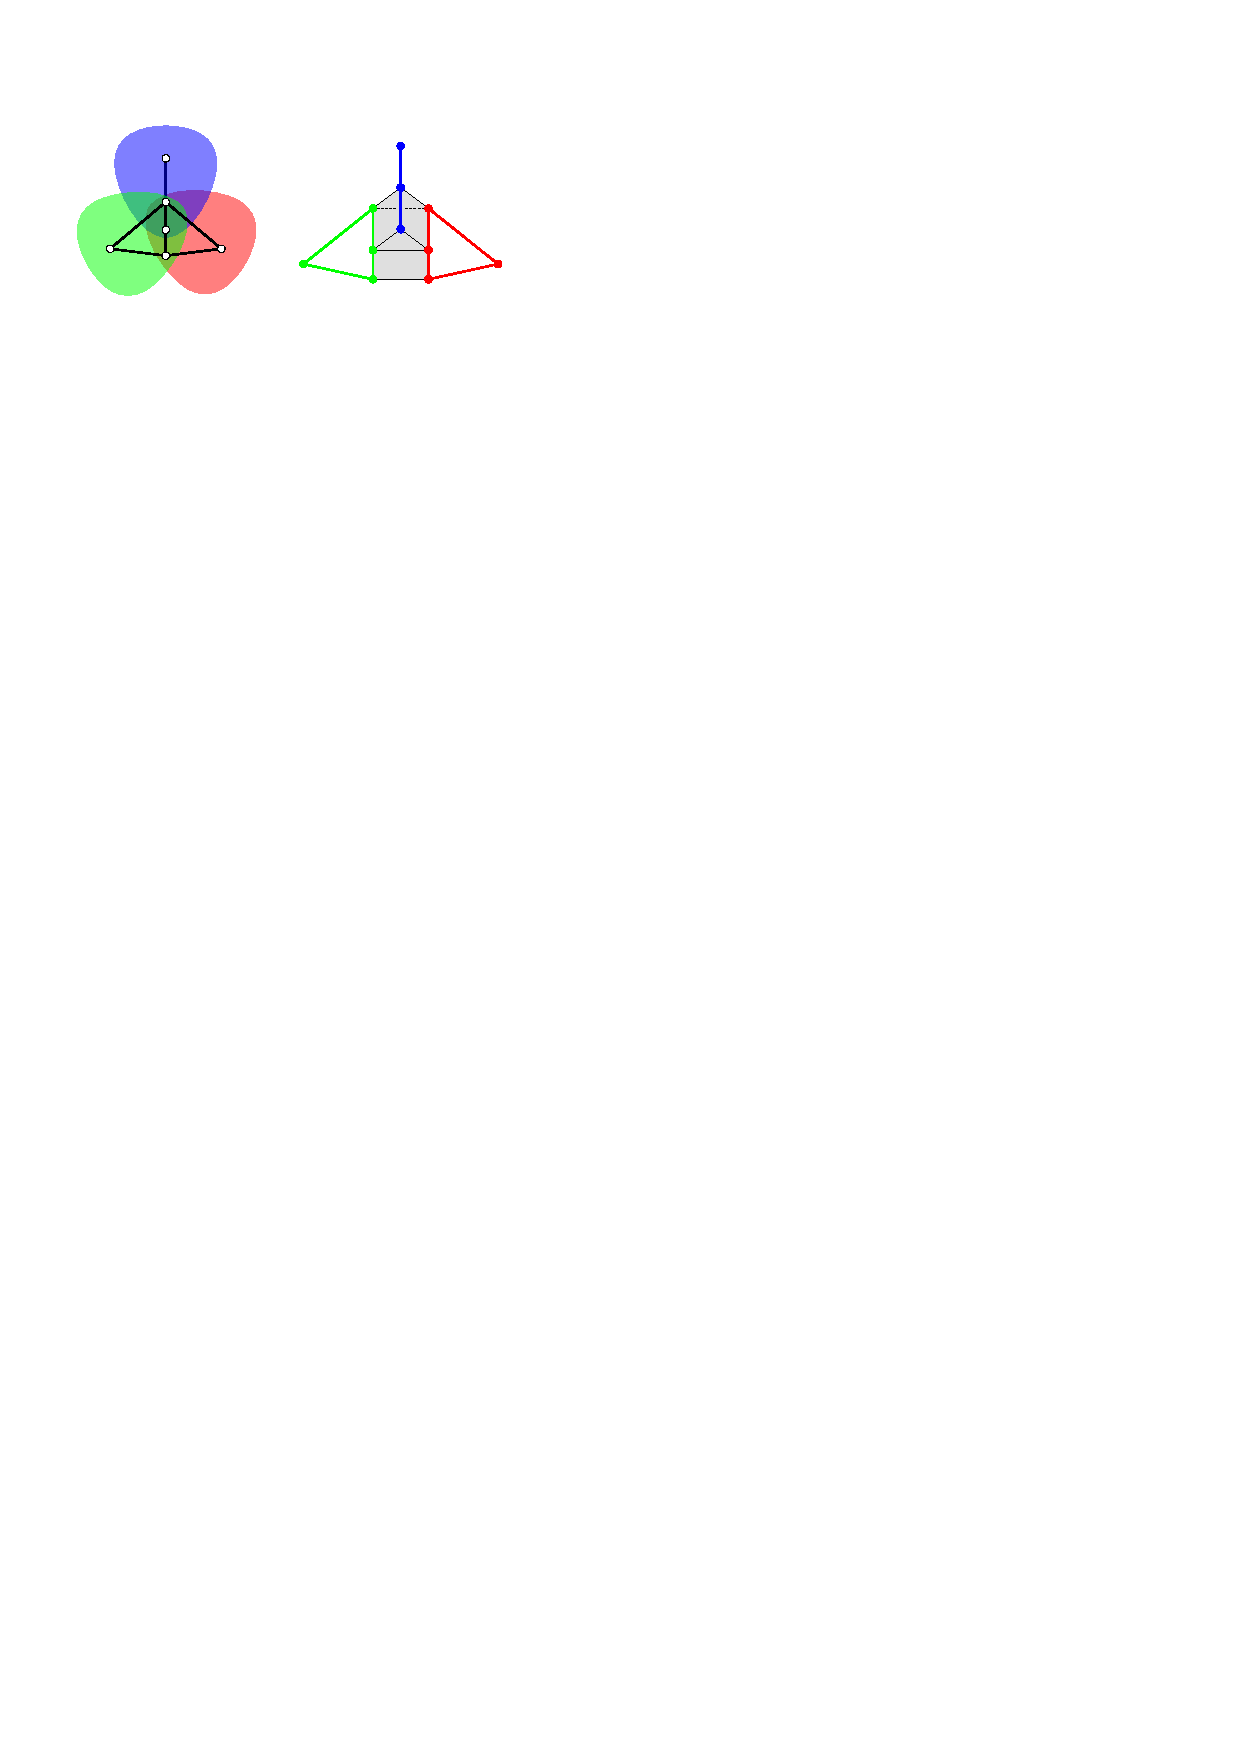
\includegraphics{figs/blowup}
    \caption{Left: Simplicial complex $K$. The subcomplexes of the cover are
             highlighted with three shaded regions.
             Right: The resulting blowup complex $K^\Cc$,
             with the disjoint subcomplexes of the cover shown in red, green, and blue.}
    \label{fig:blowup}
\end{figure}
%
Figure~\ref{fig:blowup} illustrates a simplicial complex, covered by three
subcomplexes, and the resulting blowup complex.

%In the next section we describe the chain complex structure of the blowup complex.

\paragraph{Chain complex of the blowup.}
A basis for the chain complex may be prescribed via
tensor products
$C_*(K^\Cc) = \langle \sigma \times J \mid \sigma \times J  \in K^\Cc  \rangle$
\cite[Section 4.3]{localized-homology}.
%
The tensor product structure endows the boundary operator of
the blowup complex with a useful structure.
%
The boundary of a cell $\ssx \times J \in K^\Cc$ is given by~\cite[Lemma 4]{localized-homology},
\begin{equation}
    \label{eq:blowup-boundary}
    \bdry (\ssx \otimes J) = \bdry \ssx \otimes J + (-1)^{\dim{\ssx}} \ssx \otimes \bdry J.
\end{equation}

With a boundary operator defined we may now consider the homology of the
blowup complex $\Hgr(K^\Cc)$.
%
Let $\pi: K^\Cc \to K$ denote the projection of the blowup complex onto the
first factor. This map is a homotopy equivalence~\cite{localized-homology}.
We do not define this technical term, but note that it implies that the map
$\pi^*: \Hgr(K^\Cc) \to \Hgr(K)$, induced on homology, is an isomorphism.

In moving to persistent homology, we need only specify a partial order on
the $K^\Cc$.
%
%\Remark{Filtration by the base space filtration with ties broken by the nerve dimension.}
Given a subcomplex $L \subseteq K$ of the base complex, we define the induced
subcomplex of the blowup by
\[
    L^\Cc = \bigcup\limits_{J \subseteq I} \bigcup\limits_{\ssx \in (K^J \cap L)} \ssx \times J.
\]
The projection map, $\pi_L: L^\Cc \to L$, is also a homotopy equivalence,
so the map $\pi_L^*: \Hgr(L^\Cc) \to \Hgr(L)$,
induced on homology groups, is an isomorphism.
We arrive at the main reason for using the Mayer--Vietoris blowup complex.

\begin{theorem}
A filtration $K_1 \subseteq \ldots \subseteq K_i \subseteq \ldots \subseteq K$
of the base complex $K$ induces a filtration
$K_1^\Cc \subseteq \ldots \subseteq K_i^\Cc \subseteq \ldots \subseteq K^\Cc$
of the blowup complex. Passing to homology, we get two sequences of homology
groups connected by isomorphisms,
\[
\divide\dgARROWLENGTH by2
\begin{diagram}
    \node{\Hgr(K_1)}    \arrow{e}
    \node{\ldots}       \arrow{e}
    \node{\Hgr(K_i)}    \arrow{e}
    \node{\ldots}       \arrow{e}
    \node{\Hgr(K_n)}      \\
    %
    \node{\Hgr(K_1^\Cc)}    \arrow{e}\arrow{n,r}{\pi^*_1}
    \node{\ldots}           \arrow{e}
    \node{\Hgr(K_i^\Cc)}    \arrow{e}\arrow{n,r}{\pi^*_i}
    \node{\ldots}           \arrow{e}
    \node{\Hgr(K_n^\Cc)}    \arrow{n,r}{\pi^*_n}
\end{diagram}
\]
The persistence pairs in the two sequences are the same.
\end{theorem}
\begin{proof}
    The vertical maps are isomorphisms. The projections $\pi_i$ commute
    with the inclusions, so the entire diagram commutes. Persistence
    Equivalence Theorem implies that the persistence pairs in the top and bottom
    sequences are the same.
\end{proof}
%
In other words, we can compute the persistence pairing of the filtration of $K$
from the filtration of $K^\Cc$.


%% DM: We'll make the connection in the introduction. Here it's both confusing and
%%     unnecessary. Not to mention that nerve hasn't been defined.
%We now relate this result to prior work.
%%
%Given a filtration on $K$ and a filtration on $N(\Cc)$ there are two
%induced filtration orders on $K^\Cc$. They are given by comparing
%a pair of product cells by either the factor in the base complex $K$ or its
%factor in the nerve $N(\Cc)$, breaking
%ties using the remaining factor. The former order is used in the above theorem,
%and the two orders produce different persistence diagrams.

We end this section by noting that in the filtration of $K^\Cc$,
the complex is not constructed one cell at a time, i.e., the difference between
$K^\Cc_{i+1}$ and $K^\Cc_i$ may consist of multiple cells. Within an algorithm
we make break these ties in the partial order arbitrarily.
%% DM: I'm reluctant to confuse the reader with the mention of unexplained Morse
%%      reductions. We could mention these in the conclusion.
%and while not considered in this work, one may consider exploiting morse
%reduction to reduce the computational work.

\section{Algorithm}
\label{sec:algorithm}

\begin{figure}
    \centering
    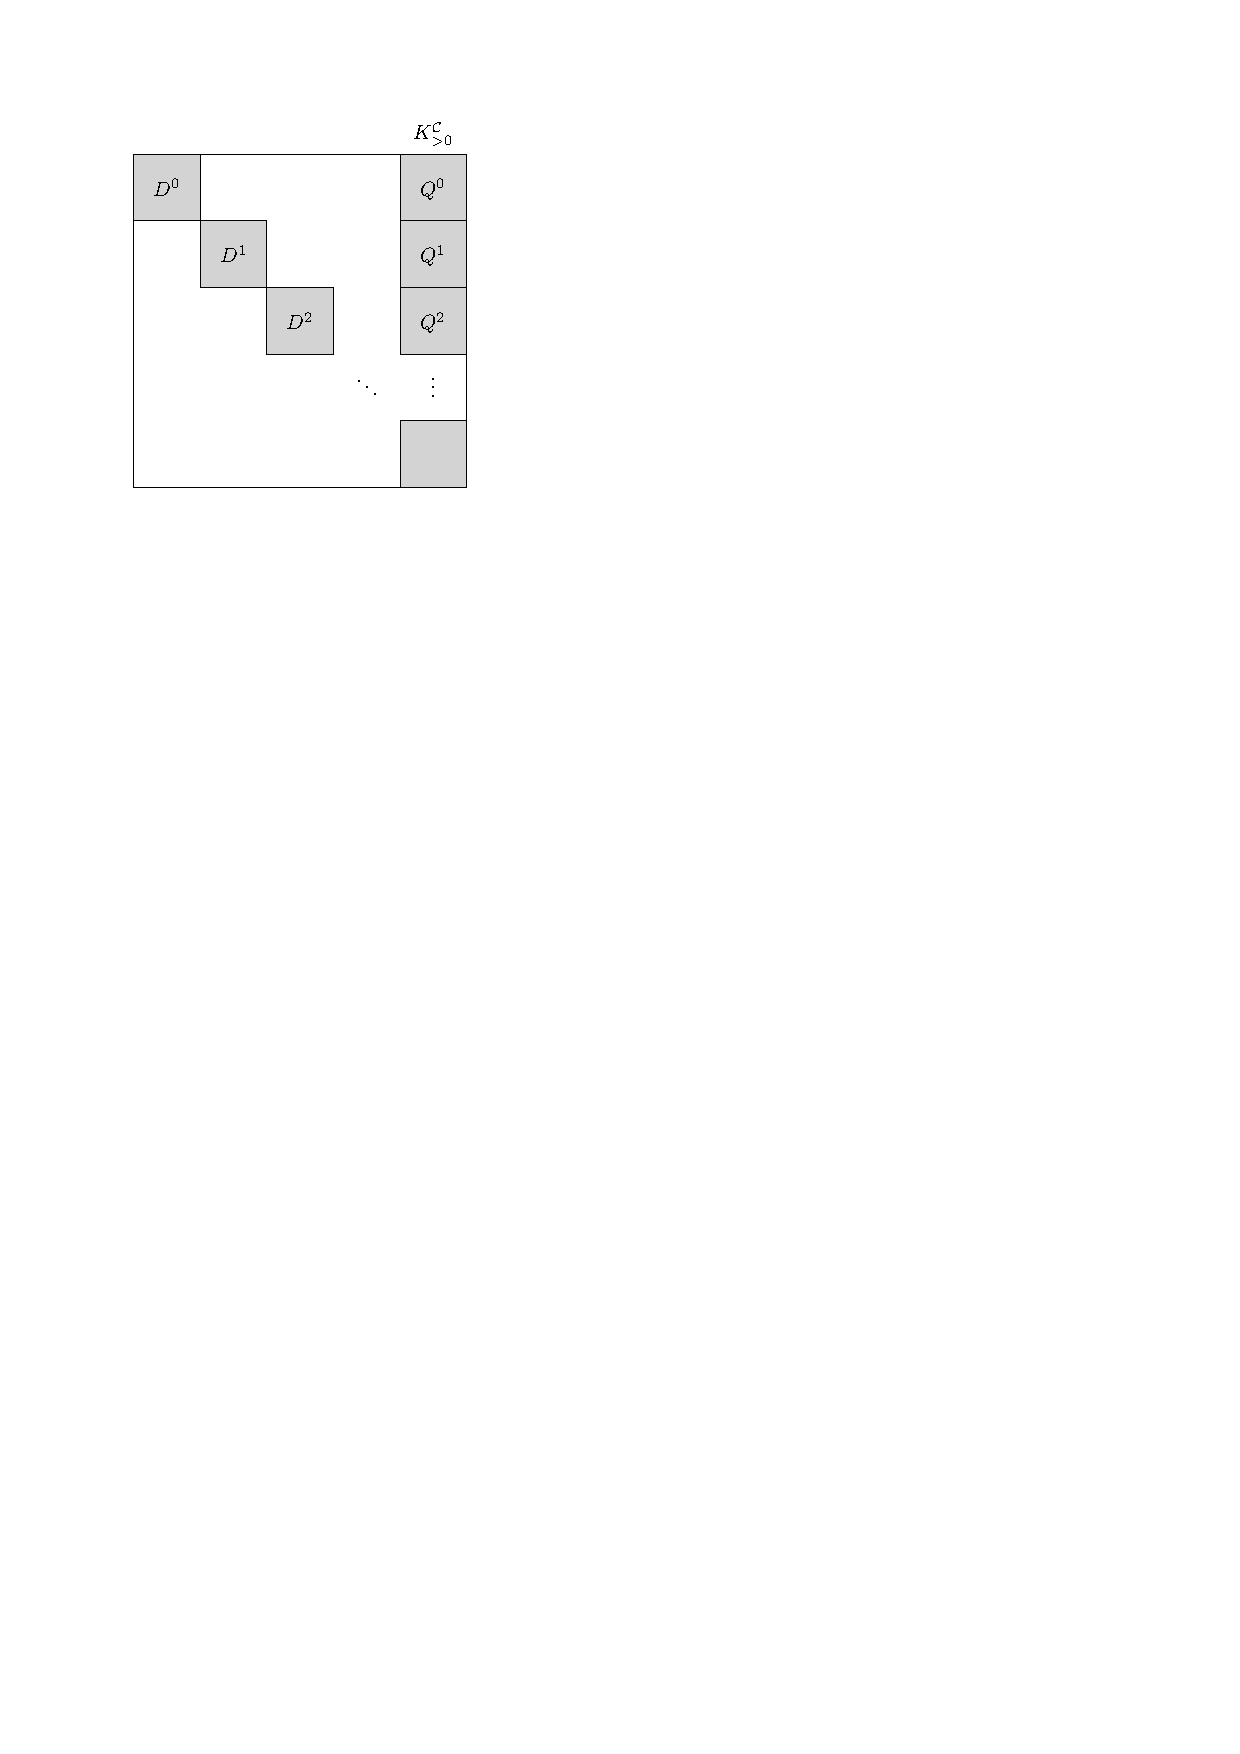
\includegraphics[page=1]{figs/blowup-boundary}
    \caption{Schematic structure of the boundary matrix of the blowup complex.
             Only shaded regions may be non-zero.}
    \label{fig:blowup-boundary}
\end{figure}

%\Remark{Boundary map of $K^C$.}
It is helpful to understand the special structure of the boundary map
\eqref{eq:blowup-boundary} in the blowup complex.
Over $\Zsp/2\Zsp$ coefficients, the boundary of a cell $\ssx \times J \in
K^\Cc$ becomes
\[
    \bdry (\ssx \otimes J) = \bdry \ssx \otimes J + \ssx \otimes \bdry J.
\]
Let the matrix $D^\Cc$ represent this boundary map, with columns and rows ordered to
respect the given filtration of $K^\Cc$. In other words, if we were to reduce
$D^\Cc$ using the $\alg{ELZ}(D^\Cc)$ algorithm, we would get the correct persistence pairing.

Suppose we reorder the columns and the rows of $D^\Cc$ as follows.
We group together the rows and the columns $\ssx \times \{ i \}$
that belong to the individual
disjoint sets of the cover (ordering them by filtration within these sets), and
we group together columns that correspond to the cells $\ssx \times J$, where the second
factor $J$ has dimension higher than 0, again ordering by filtration within those
columns. Figure~\ref{fig:blowup-boundary} shows this structure schematically:
$D^0, D^1, D^2$ denote the sub-matrices of the disjoint sets, i.e., the columns
of $D^i$ record the boundaries of the cells $\ssx \times \{ i \}$,
where $\ssx \in K^i$.
The right-most block of shaded columns represents the cells with
higher-dimensional second factor, i.e., the cells $\ssx \times J$, where
$\dim J > 0$.
We denote by $Q^i$ their sub-blocks that fall into the rows
$\ssx \times \{ i \}$ that correspond to the cells of the disjoint union.
%
Notice that outside the shaded regions in Figure~\ref{fig:blowup-boundary}, the
matrix is necessarily zero.

We observe that because we've ordered the cells within the blocks by filtration,
we may carry out operations within the blocks --- column operations from left to
right, row operations from bottom up --- without violating the column and row
order within the original matrix $D^\Cc$.

Accordingly, we may column-reduce individual matrix blocks independently,
decomposing $D^i = R^i U^i$ using $\alg{ELZ}(D^i)$ algorithm. We may further
row-reduce matrices $R^i$, getting decomposition $D^i = S^i P^i U^i$
using $\alg{Sparsify}(R^i)$ algorithm.
(The matrix $P^i$ has an immediate interpretation: it records the persistence pairs
in the restriction of the input filtration to the cover set $K^i$.)
To be consistent in the full boundary matrix $D^\Cc$, we must perform the row operations on the full rows, thus replacing
blocks $Q^i$ with blocks $S^i Q^i$.
We call the resulting matrix $T'$, see Figure~\ref{fig:blowup-boundary-reduced}.

\begin{figure}
    \centering
    \includegraphics[page=2]{figs/blowup-boundary}
    \caption{The matrix $T'$, formed out of the boundary matrix of the blowup complex
             after the initial column and row reductions.}
    \label{fig:blowup-boundary-reduced}
\end{figure}

%\Remark{Explain the structure of the coboundary of a cell.}
It is helpful to note the structure of the blocks $Q_i$.
Which blowup cells have the base cells of the disjoint union,
$\ssx \times \{ i \}$, in their boundary?
First of all, these are the cells $\tsx \times \{ i \}$,
with $\ssx \in \bdry \tsx$; the first factor of their boundary map
\eqref{eq:blowup-boundary} consists of the cells $\ssx \times \{ i \}$.
Their boundaries define the columns of the sub-matrices $D^i$.
The second type of a cell that has $\ssx \times \{ i \}$ in
its boundary are the cells $\ssx \times \{ i, j \}$, where cover set $K^j$
intersects cover set $K^i$. The part of the row of cell $\ssx \times \{ i \}$
that falls into the block $Q^i$ has non-zero entries in the columns of such
cells. These are the only two possibilities allowed by the boundary
formula~\eqref{eq:blowup-boundary}.
Most rows of matrices $Q^i$ are zero, since only cells that fall into more than
one cover set have non-zero entries in the columns of $Q^i$.

Now, if we reorder the columns and the rows of the matrix $T'$ back into the
original filtration order, call the resulting matrix $T$, and reduce it using
algorithm $\alg{ELZ}(T)$, the $\low$ map on the resulting matrix $R_T$ will
produce the correct persistence pairing.

\begin{theorem}
    $(i, j)$ is a pair in $\Hgr(K^\Cc_0) \to \ldots \to \Hgr(K^\Cc_n)$ if and
    only if $\low R_T[j] = i$.
    %\Remark{The statement needs to deal with the fact that multiple changes occur per
    %        step of the blowup filtration.}
\end{theorem}
\begin{proof}
    We pad and reorder the rows and columns of matrices $S^i$ and $U^i$ so that
    they match the original blowup boundary matrix $D^\Cc$. (The padding is to
    identity, i.e., the newly added rows and columns have 1s on the diagonal, so
    the padded matrices remain invertible upper-triangular.)
    %Equivalently, the padded matrices preserve the newly added columns and rows.
    Since the operations in matrices $D^i$ respected the filtration order, the
    padded matrices $S^i$ and $U^i$ remain invertible upper-triangular.
    Therefore, so are their products $S = S^0 \cdot S^1 \cdot \ldots$ and
    $U = U^0 \cdot U^1 \cdot \ldots$
    Therefore,
    the first set of independent reductions results in the decomposition
    $D^\Cc = S T U$, with $T$ appropriately reordered. Now reducing the matrix $T$
    using $\alg{ELZ}(T)$ algorithm produces decomposition
    $T = R_T U_T$, where $R_T$ is reduced and $U_T$ is invertible upper-triangular.
    Therefore, the complete decomposition is $D^\Cc = S R_T (U_T U)$, and
    Lemma~\ref{lem:pairing-uniqueness} implies the claim.
\end{proof}


\paragraph{Parallel setup.}
If we have $p$ cover sets, i.e., $p = \card I$, then we can split the initial
operations $\alg{ELZ}(D^i)$ and $\alg{Sparsify}(R^i)$ between $p$ processors.
The final reduction $\alg{ELZ}(T)$ can be performed by either one of them.
%
If all the processors share the same memory, we may be satisfied with this
solution, although we can perform a little more work in parallel, as explained
in Section~\ref{sec:hierarchy}.

If the memory is distributed, the separate bits of information
$P^i$ and $S^i Q^i$, necessary for the final reduction, need to be brought to a
single processor. In Section~\ref{sec:hierarchy} we explain how this operation
can be performed using a binary reduction. Meanwhile, we mention a simple, but
important optimization: it suffices to send only those rows of $P^i$ that are
not zero in $S^i Q^i$; the rows that are zero in $S^i Q^i$ record the pairs that
will not change.


\section{Cascade}
\label{sec:cascade}

So far it is unclear why we performed the seemingly unnecessary sparsification
step, converting matrices $R^i$ into matrices $P^i$.
The sparsification is advantageous since it reduces the potentially quadratic
size of matrices $R^i$ down to the linear size of matrices $P^i$.
In the distributed setting, this means
less data to send to the processor responsible for the final reduction.
But there is another advantage. The combined matrix $T$ has a special sparsity
pattern.
%
This structure allows for a faster reduction even using the standard
$\alg{ELZ}(T)$ algorithm.
In addition, with a little extra work, presented in
%In this section,
algorithm $\alg{Cascade}(T)$, Algorithm~\ref{alg:cascade},
we can preserve this structure throughout the computation and thus gain
efficiency both in time and in space.

Suppose there are $n = \sum_{i \in I} \card K^i$ cells in the blowup complex
that fall into the disjoint union, and there are $m$ cells with
higher-dimensional second factor,
$m = \card \{ \ssx \times J \mid \ssx \times J \in K^\Cc, \dim J > 0 \}$.
We assume $m < n$.
Then reducing the matrix $T$ using
$\alg{ELZ}(T)$ algorithm takes, in the worst case, $\bigO{n^2 m}$ time and
$\bigO{n^2}$ space.
(The reason why the time complexity is tighter than $\bigO{n^3}$ is similar to
the analysis in the proof of Theorem~\ref{thm:complexity} below.)

The matrix $T$ has special structure, see Figure~\ref{fig:cascade}.
The $n$ columns of the disjoint union
are formed by matrices $P^i$, which have at most one non-zero entry per column.
We call such columns \emph{ultra-sparse}. The remaining $m$ columns are
\emph{dense}. Given such a matrix, with $n$ ultra-sparse columns and $m$ dense
columns, we can reduce it as follows.

We iterate over the rows of the matrix $T$ from the bottom up, and consider the
columns whose lowest ones fall into a given row. Let $J$ be the set of their
indices.
At most one such column can be ultra-sparse because the matrices $P^i$ are reduced.
Let $j$ denote the first column in the set $J$. We can subtract it from every
other column in $J$.  If one of those columns is ultra-sparse and column $j$ is
dense, then the ultra-sparse column becomes dense. To keep the number of dense
columns constant, we subtract the current row (which after the column operations
has a single non-zero in column $j$) from every other row with a non-zero entry
in column $j$. In other words, we zero out column $j$, making it ultra-sparse.
%
Algorithm~\ref{alg:cascade} performs the described operations.

\begin{figure}
    \centering
    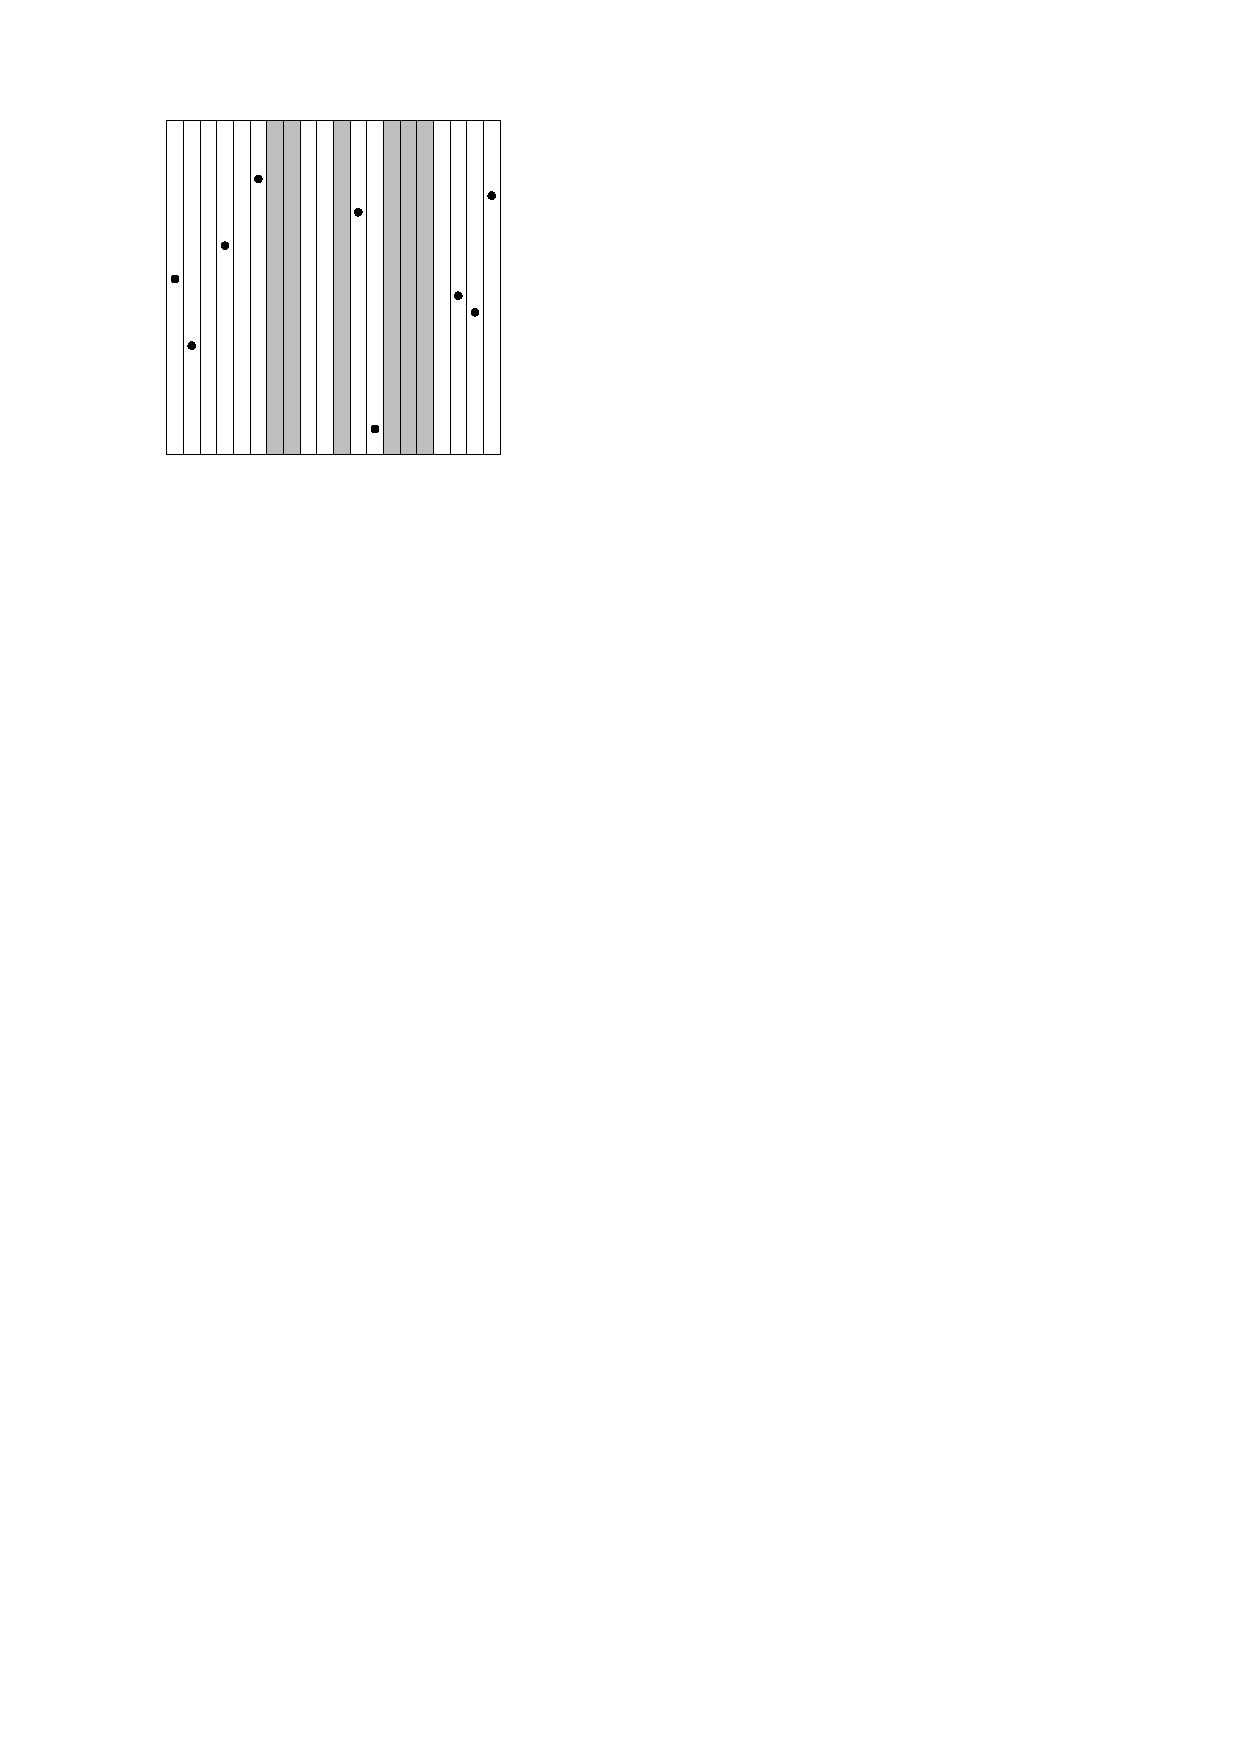
\includegraphics{figs/almost-permutation}
    \caption{Structure of the matrix $T$ prior to the reduction. Shaded columns are
             dense. The rest of the columns are ultra-sparse, they have at most
             one non-zero entry.}
    \label{fig:cascade}
\end{figure}

\begin{algorithm*}
$\alg{Cascade}(T):$
\begin{algorithmic}
    \ForAll{rows $\row{T}{i}$, from bottom up}
        \State $J$ = columns with the lowest non-zero entry in row $\row{T}{i}$
        \State $j = \min J$
        \ForAll{$j' \in J, j' > j$}
            \State subtract $\col{T}{j}$ from $\col{T}{j'}$
        \EndFor
        \ForAll{$i' < i$ with $T[i,j] \neq 0$}
        \State subtract $\row{T}{i}$ from $\row{T}{i'}$     \Comment{zero out all but the lowest entry of column $\col{T}{j}$}
        \EndFor
    \EndFor
\end{algorithmic}
\caption{Cascade algorithm for the reduction of the matrix $T$ with ultra-sparse columns.}
\label{alg:cascade}
\end{algorithm*}


Since $\alg{Cascade}(T)$ performs operations from left to right and from bottom
up, Lemma~\ref{lem:pairing-uniqueness} immediately implies its correctness.

\eject
\begin{theorem}
    Lowest ones of the matrix $T$ reduced using $\alg{Cascade}(T)$ algorithm produce
    the correct pairing of the sequence of homology groups,
    $\Hgr(K_0^\Cc) \to \ldots \Hgr(K_n^\Cc)$.
\end{theorem}

What is the worst case complexity of $\alg{Cascade}(T)$?

\begin{theorem}
    \label{thm:complexity}
    $\alg{Cascade}(T)$ algorithm reduces the matrix $T$ with $n$ ultra-sparse and
    $m$ dense columns in time $\bigO{n^2 m}$, while keeping its size $\bigO{nm}$.
\end{theorem}
\begin{proof}
    The initial number of nonzero elements in the matrix $T$ is in $\bigO{(n + m) m + n} = \bigO{nm}$.
    Since the number of dense columns is kept constant (or, more accurately, it
    never increases) thanks to the row operations that clear out column $j$, the
    space used during the cascade remains in $\bigO{nm}$.

    It takes $\bigO{n+m}$ time to add two dense columns, or to add a dense
    column to a sparse column. How many such operations are there?
    At most $m$ per row. There are $n+m$ rows, for a total of
    $\bigO{(n+m)^2 m} = \bigO{n^2 m}$ operations.
\end{proof}


\section{Hierarchy}
\label{sec:hierarchy}

So far we have considered the case of a single cover of the domain, a collection
of simplicial complexes $\Cc = \{ K^i \}_I$ with domain $K = \bigcup \Cc$. But in many
applications, it is natural to build a hierarchy of such covers. For example, if
the domain $K$ triangulates a cube or a flat torus (a cube with periodic
boundary conditions), both exceedingly common scenarios for
simulation data, one can build a refinement of covers following an oct-tree
partition of the cube. The cubes at each level of the oct-tree become the cover
sets.
(Technically, the cover sets are the closures of the subcomplexes of $K$ that
intersect those cubes.)

Given such a hierarchy, it becomes possible to follow the standard reduction
pattern and merge sets together in pairs (or, more generally, in small groups) and
thus to extend the amount of useful work a processor can do. It also limits how
many dense columns $m$ a single processor has to handle at once.
%
Consider the prototypical oct-tree example.
If we have $p = 8^k$ processors and descend down to the $k$-th level in the
tree, we end up with $p$ cubes and $m = 3 \cdot 2^k \cdot c$ shared simplices,
where $c$ is the number of simplices in a side of the cube.
On the other hand, if we merge the cubes in pairs (proceeding to a higher level
in the oct-tree after each merge), $m$ never exceeds $c$, the size of the
initial cut that splits the domain into two.

We can abstract the hierarchical partition of an oct-tree as a nested collection of
covers $\Cc_0, \Cc_1, \ldots$, such that $K = \bigcup \Cc_0 = \bigcup \Cc_1 = \ldots$
and every cover set $L^i \in \Cc_a$ is contained in exactly one cover set
$K^j \in \Cc_{a-1}$, $L^i \subseteq K^j$.

%\Remark{Explain the relationship between the boundary matrices. I.e., how to get
%        to one from the other.}
Consider the structure of the boundary matrix for two consecutive levels in the
cover, illustrated in Figure~\ref{fig:hierarchy}. Suppose at level $i+1$ the
cover consists of four sets, $\Cc_{i+1} = \{ K^1, K^2, K^3, K^4 \}$, and at level
$i$ the cover consists of two sets $\Cc_i = \{ K^1 \cup K^2, K^3 \cup K^4 \}$.
%
The procedure outlined in
Sections~\ref{sec:algorithm}~and~\ref{sec:cascade} would operate independently
on the matrices $D^1, D^2, D^3,$ and $D^4$ (on four different processors). The first
two results would then be combined by first performing row updates on the matrices $Q^1$ and
$Q^2$, then reordering the matrix and reducing it using the {\bf Cascade}
algorithm.
The second pair of results would be combined similarly.
The two combined matrices contain the same information as the reduced boundary
matrices $R^{12}$ and $R^{34}$ for the cover sets $K^1 \cup K^2$
and $K^3 \cup K^4$ at level $i$. We could proceed with the algorithm at level
$i$, with one caveat: the higher rows (the second to last column in the figure)
involved in the combination did not get updated during the execution of {\bf
Sparsify} and {\bf Cascade} algorithms. The fix is straight-forward: when
processing any given level of the cover, we perform the row operations on the
full rows, rather than on their restriction to the given level.
The only information necessary to construct such rows is knowing which sets of
the cover contain any given simplex.

\begin{figure}
    \centering
    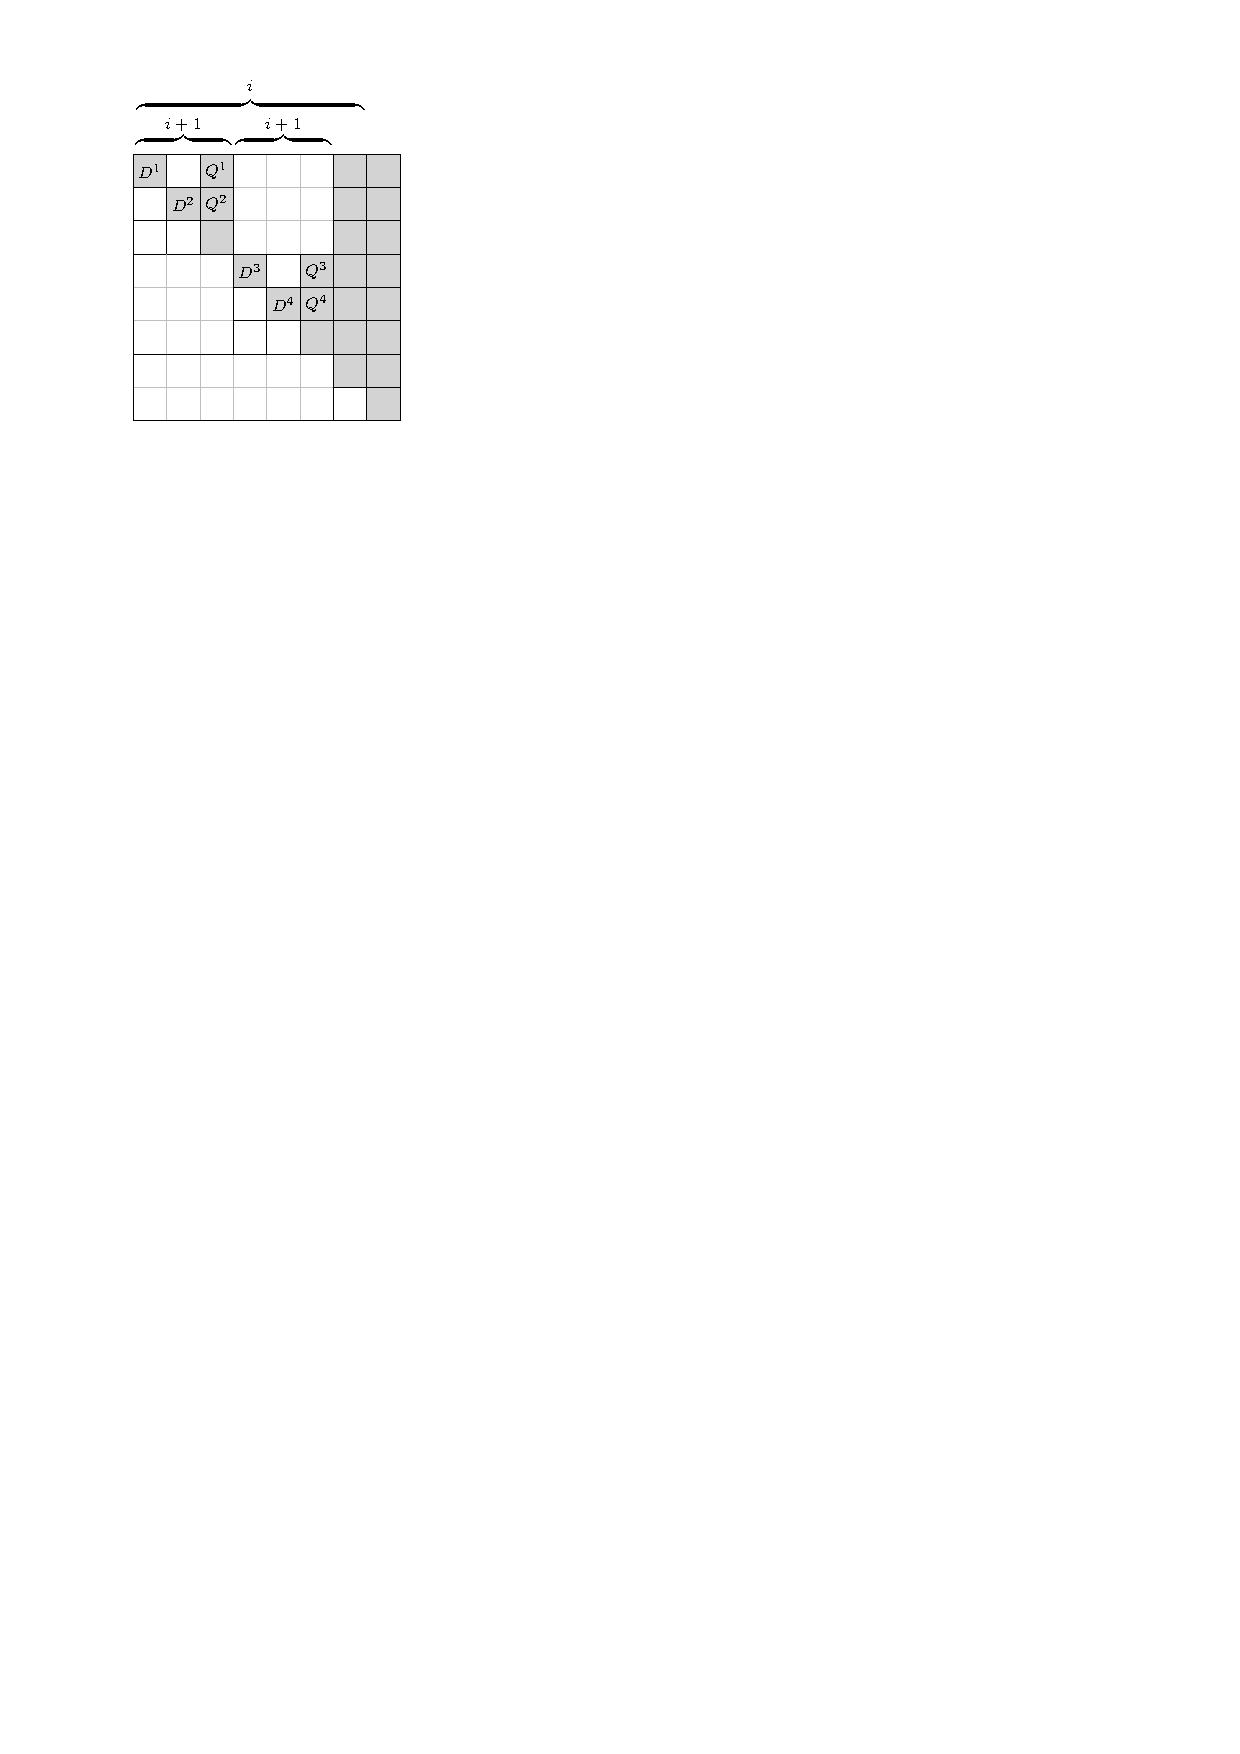
\includegraphics{figs/hierarchy}
    %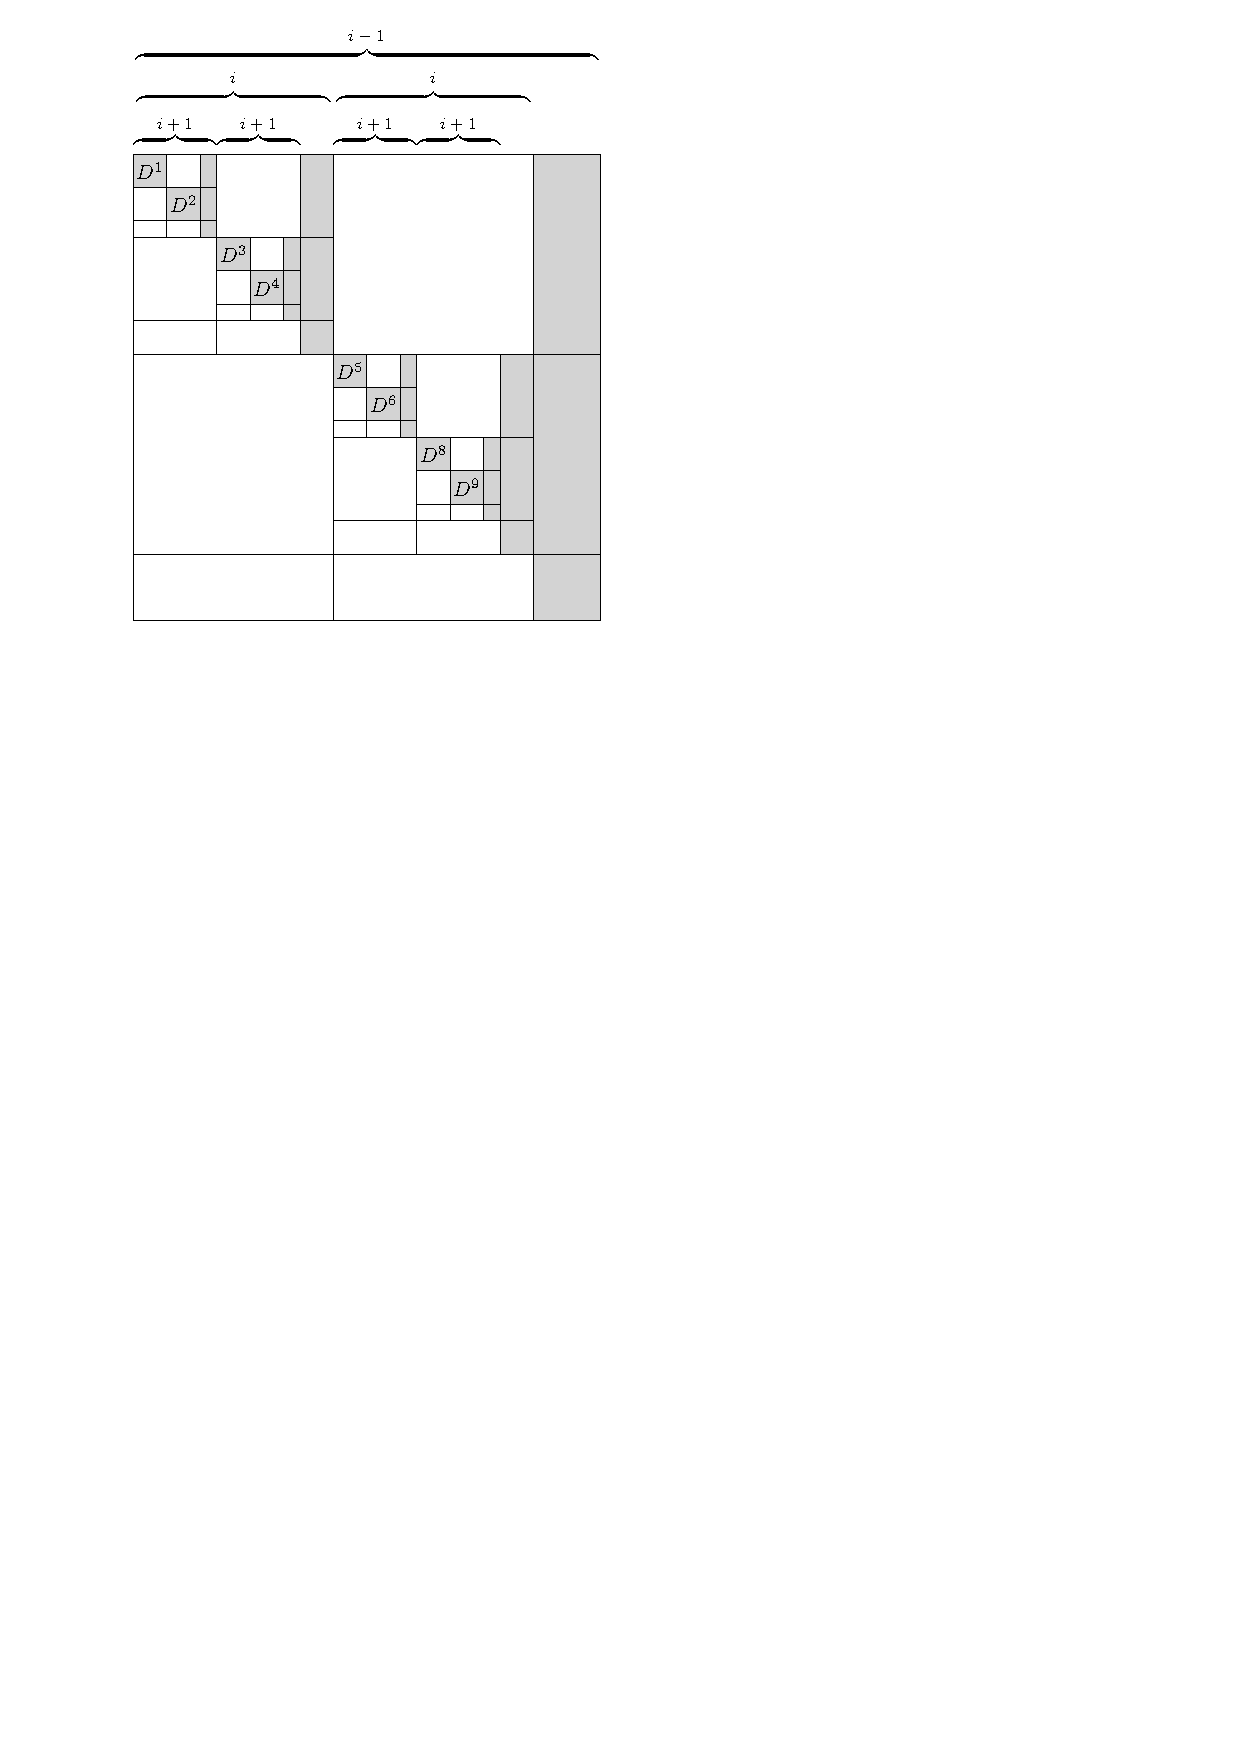
\includegraphics[width=.46\textwidth]{figs/boundary-hierarchy}
    \caption{The structure of the boundary matrix for three consecutive levels of
             the hierarchy.}
    \label{fig:hierarchy}
\end{figure}


\eject
\section{Experiments}
\label{sec:experiments}

We have implemented the described algorithm on top of MPI, and ran a strong
scaling experiment on Edison supercomputer at the National Energy Research
Scientific Computing Center (NERSC). Edison is a Cray XC30 system; its
individual compute nodes have 24 Intel `Ivy Bridge' processor cores, at 2.4 GHz,
with 64KB and 256KB of L1 and L2 cache, respectively; the 24 cores share 64GB of RAM.

Our input is a snapshot of a combustion simulation, a $256^2 \times 512$ scalar
field.
%of density \Remark{of what} during a burning of methane.
The input
simplicial complex is a Freudenthal triangulation of the grid,
with $\sim 870 \cdot 10^6$ simplices. It is covered hierarchically via an
oct-tree.

Figure~\ref{fig:times} and Table~\ref{tbl:times} summarize the running times
(wallclock as reported by the PBS job resource manager).
Going from 8 to 32 processes we see a near
perfect scaling, with another improvement by a factor of $\sim 1.5$ going from
32 to 64 processes. But then the returns diminish rapidly. The behavior is not
surprising: past 64 processes the binary reduction used to merge
different cover sets is top-heavy, i.e., it's dominated by the merge of the
information from the final two sets. As a result, adding more processes only
speeds up the initial computation, which is already plenty fast.

\pgfplotstableread{data/plt07895.dat}\pltCombustionMed

\begin{figure}
    \centering
    \begin{tikzpicture}
    \begin{axis}[
                    %ybar,
                    %xtick=data,
                    ymode=log,
                    %log basis y=2,
                    tick align=inside,
                    %ymax=100,
                    ymin=580,
                    symbolic x coords={8,16,32,64,128,256,512},
                    height=3in,
                    width=.5\textwidth,
                    xlabel={Number of processes},
                    ylabel={Seconds},
                ]
        \addlegendentry{\hspace{.3in} Persistence ($256^2 \times 512$):}
        \addplot+[] table[x=proc,y=time]
                  {\pltCombustionMed};
        \addlegendentry{\hspace{.3in}Perfect scaling:}
        %\addplot+[dashed, red, mark=none] table[x=proc,y=perfect]
        %          {\pltCombustionMed};
        \addplot+[dashed, red, mark=none] coordinates
                  {
                      (8,  4096)
                      (16, 2048)
                      (32, 1024)
                      (64, 512)
                  };
    \end{axis}
    \end{tikzpicture}

    \caption{Times to compute persistence diagram for the $256^2 \times 512$
             combustion data set. The measurements are in Table~\ref{tbl:times}.}
    \label{fig:times}
\end{figure}

\begin{table}
    \centering
    \pgfplotstabletypeset
    [
        every head row/.style={
            before row={
                \toprule
            },
            after row=\midrule,
        },
        columns={proc, time},
        columns/proc/.style         ={column name=processors, int detect, column type={r}},
        columns/time/.style         ={column name=seconds, fixed, column type={|r}},
    ]
    {\pltCombustionMed}
    \caption{Times to compute persistence diagram for the $256^2 \times 512$
             combustion data set. The data is presented visually in
             Figure~\ref{fig:times}.}
    \label{tbl:times}
\end{table}

What is worse is what the figure does not show. We have tried our code on larger
data sets, but ran out of memory because the merge reduction is dominated by its
final stages. Although the $(n+m)$ term in the space analysis of the
\alg{Cascade} algorithm is a gross worst-case overestimate, the growth of this
term does follow the growth of $n$, the size of the domain, in many practical
examples. So our technique does not solve the memory limitations of the
persistence algorithm for the large data set. We address this issue in the next
section.


\eject
\section{Conclusion}

%\Remark{Combining with the spectral sequence algorithm.}
Despite the evident limitation of a merge reduction, we believe our theoretical
results have a place as building blocks of a practical parallel persistence algorithm.
In particular, an interesting (and, we believe, promising) research direction is
combining the domain decomposition approach of our paper with the spectral sequence
algorithm~\cite{EH-book,dipha}.
%
One could initially distribute the data with respect to a domain decomposition:
often such a distribution is either very cheap to compute, or entirely
free in the cases when the data is supplied already decomposed directly from a simulation code,
or it is stored decomposed (for I/O-efficiency). In this case, much processing
could be performed on the individual chunks of the data; this part of our
algorithm scales perfectly. Then, when combining the individual results, one
could redistribute the remaining matrix (the input to the $\alg{Cascade}$
algorithm) with respect to the diagonal block partition of the spectral sequence
algorithm. This way we could limit the space needed on any given processor.


%\Remark{Open issues: translating this construction to the cohomology algorithm;
%        understanding which optimizations are applicable and useful.}
Another important research topic is adapting our algorithm to the computation of
persistent cohomology. Although the resulting pairing is the same, algorithms
that keep track of cocycles rather than cycles have been reported to perform
significantly better in practice~\cite{dualities,compressed-annotation-matrix}.
On the other hand, they are built around tracking the matrix $U^{-1}$ in the $D=RU$
decomposition, while the algorithm that we've presented depends on manipulating
the matrix $R$.

Similarly, it would be fruitful to understand the relationship of our algorithm
to various practical optimizations~\cite{parallel-phat}.
Unexpectedly to us, the original optimization~\cite{ELZ02} that removes negative
simplices from the columns of the matrix $R$ cannot be used in our context.
The reason is that a simplex that is
negative in the filtration of a cover subcomplex $K^i$ may be positive in the
filtration of the entire space $K$.
On the other hand, if a simplex creates a cycle in the filtration of $K^i$
(i.e., it is positive), it must be positive in the filtration of the entire $K$.
Thus the clearing optimization of Chen and Kerber~\cite{clearing-optimization}
is readily applicable.


%\eject
\clearpage
\begin{thebibliography}{99}

\bibitem{ELZ02}
\textsc{Herbert Edelsbrunner, David Letscher, and Afra Zomorodian.}
\newblock Topological Persistence and Simplification.
\newblock \emph{Proceedings of the Annual Symposium on Foundations of Computer Science}, pages 454--463, 2000.
\newblock \emph{Discrete and Computational Geometry,} \textbf{28}:511--533, 2002.

\bibitem{CZ05}
\textsc{Afra Zomorodian and Gunnar Carlsson.}
\newblock Computing Persistent Homology.
\newblock \emph{Discrete and Computational Geometry,} \textbf{33}:249--274, 2005.

\bibitem{persistence-clustering}
\textsc{Fr\'ed\'eric Chazal, Leonidas J.\ Guibas, Steve Y.\ Oudot, Primo\v z \v Skraba.}
\newblock Persistence-Based Clustering in Riemannian Manifolds.
\newblock \emph{Journal of the ACM}, \textbf{60}, 2013.

\bibitem{circular-coordinates}
\textsc{Vin de Silva, Dmitriy Morozov, Mikael Vejdemo-Johansson.}
\newblock Persistent Cohomology and Circular Coordinates.
\newblock \emph{Discrete and Computational Geometry}, \textbf{45}:737--759, 2011.

\bibitem{SW-measuring-shape}
\textsc{Robert D.~MacPherson and Benjamin Schweinhart.}
\newblock Measuring Shape with Topology.
\newblock \emph{Journal of Mathematical Physics,} \textbf{53}, 2012.

\bibitem{cosmic-web}
%R. van de Weygaert, G. Vegter, H. Edelsbrunner, B. J. T. Jones, P. Pranav, C. Park, W. A. Hellwing, B. Eldering, N. Kruithof, E. G. P. Box, J. Hidding, J. Feldbrugge, E. ten Have, M. van Engelen, M. Caroli and M. Teillaud.
\textsc{Rien van de Weygaert et al.}
\newblock Alpha, Betti and the megaparsec Universe: on the topology of the cosmic web.
\newblock \emph{Trans. Comput. Sci. XIV}, pages 60--101, 2011.

\bibitem{CSE-curves}
\textsc{David Cohen-Steiner and Herbert Edelsbrunner.}
\newblock Inequalities for the curvature of curves and surfaces.
\newblock \emph{Foundations of Computational Mathematics}, \textbf{7}:391--404, 2007.

\bibitem{klein-bottle}
\textsc{Gunnar Carlsson, Tigran Ishkhanov, Vin de Silva, Afra Zomorodian.}
\newblock On the Local Behavior of Spaces of Natural Images.
\newblock \emph{International Journal of Computer Vision}, \textbf{76}:1--12, 2008.

\bibitem{EH-survey}
\textsc{Herbert Edelsbrunner and John Harer.}
\newblock Persistent homology --- a survey.
\newblock \emph{Surveys on Discrete and Computational Geometry. Twenty Years Later.}, pages 257--282, 2008.

\bibitem{ph-theory-applications}
\textsc{Herbert Edelsbrunner and Dmitriy Morozov.}
\newblock Persistent homology: theory and practice.
\newblock \emph{Proceedings of European Congress of Mathematics}, pages 31--50, 2012.

\bibitem{Ghrist-survey}
\textsc{Robert Ghrist.}
\newblock Barcodes: The persistent topology of data.
\newblock \emph{Bulletin of the American Mathematical Society}, \textbf{45}:61--75, 2007.

\bibitem{Weinberger-survey}
\textsc{Shmuel Weinberger.}
\newblock What is\ldots Persistent Homology?
\newblock \emph{Notices of the American Mathematical Society}, \textbf{58}:36--39, 2011.

\bibitem{Gunnar-survey}
\textsc{Gunnar Carlsson.}
\newblock Topology and data.
\newblock \emph{Bulletin of the American Mathematical Society}, \textbf{46}:255--308, 2009.

\bibitem{persistence-mmt}
\textsc{Nikola Milosavljevi\'c, Dmitriy Morozov, and Primo\v z \v Skraba.}
\newblock Zigzag persistent homology in matrix multiplication time.
\newblock \emph{Proceedings of the Annual Symposium on Computational Geometry,} pages 216--225, 2011.

\bibitem{persistence-lower-bound}
\textsc{Herbert Edelsbrunner and Salman Parsa.}
\newblock On the computational complexity of Betti numbers: reductions from matrix rank.
\newblock \emph{Proceedings of the Annual Symposium on Discrete Algorithms}, pages 152--160, 2014.

\bibitem{output-sensitive-persistence}
\textsc{Chao Chen and Michael Kerber.}
\newblock An output-sensitive algorithm for persistent homology.
\newblock \emph{Computational Geometry: Theory and Applications,} \textbf{46}:435--447, 2013.

\bibitem{dualities}
\textsc{Vin de Silva, Dmitriy Morozov, Mikael Vejdemo-Johansson.}
\newblock Dualities in Persistent (Co)Homology.
\newblock \emph{Inverse Problems}, \textbf{27}, 2011.

\bibitem{compressed-annotation-matrix}
\textsc{Jean-Daniel Boissonnat, Tamal K.~Dey, Cl\'ement Maria.}
\newblock The Compressed Annotation Matrix: An Efficient Data Structure for Computing Persistent Cohomology.
\newblock \emph{Proceedings of European Symposium on Algorithms}, pages 695--706, 2013.

\bibitem{clearing-optimization}
\textsc{Chao Chen and Michael Kerber.}
\newblock Persistent Homology Computation With a Twist.
\newblock \emph{Proceedings of the European Workshop on Computational Geometry}, 2011.

\bibitem{parallel-phat}
\textsc{Ulrich Bauer, Michael Kerber, Jan Reininghaus.}
\newblock Clear and Compress: Computing Persistent Homology in Chunks.
\newblock \emph{Topological Methods in Data Analysis and Visualization III}, pages 103-117, 2014.

\bibitem{dipha}
\textsc{Ulrich Bauer, Michael Kerber, Jan Reininghaus.}
\newblock Distributed Computation of Persistent Homology.
\newblock \emph{Proceedings of Algorithm Engineering and Experiments (ALENEX)},  2014.

\bibitem{zzph}
\textsc{Gunnar Carlsson, Vin de Silva, Dmitriy Morozov.}
\newblock Zigzag Persistent Homology and Real-valued Functions.
\newblock \emph{Proceedings of the Annual Symposium on Computational Geometry}, pages 247--256, 2009.

\bibitem{MV-spectral-sequence}
\textsc{David Lipsky, Primo\v z \v Skraba, Mikael Vejdemo-Johansson.}
\newblock A spectral sequence for parallelized persistence.
\newblock arXiv:1112.1245, 2011.

\bibitem{localized-homology}
\textsc{Afra Zomorodian and Gunnar Carlsson.}
\newblock Localized Homology.
\newblock \emph{Computational Geometry: Theory and Applications}, \textbf{41}:126--148, 2008.

\bibitem{multicore-homology}
\textsc{Ryan H.~Lewis and Afra Zomorodian.}
\newblock Multicore Homology via Mayer Vietoris.
\newblock arXiv:1407.2275, submitted to \emph{Computational Geometry: Theory and Applications}, 2014.

\bibitem{distributed-merge-trees}
\textsc{Dmitriy Morozov and Gunther Weber.}
\newblock Distributed Merge Trees.
\newblock \emph{Proceedings of the Annual Symposium on Principles and Practice of Parallel Programming},
          pages 93--102, 2013.

\bibitem{vineyards}
\textsc{David Cohen-Steiner, Herbert Edelsbrunner, and Dmitriy Morozov.}
\newblock Vines and Vineyards by Updating Persistence in Linear Time.
\newblock \emph{Proceedings of the Annual Symposium on Computational Geometry,} pages 119--126, 2006.

\bibitem{EH-book}
\textsc{Herbert Edelsbrunner and John Harer.}
\newblock \emph{Computational Topology: an Introduction.}
\newblock AMS Press, 2010.

\bibitem{Hatcher}
\textsc{Allen Hatcher.}
\newblock \emph{Algebraic Topology}.
\newblock Cambridge University Press, 2002.

\bibitem{classifying-spaces}
\textsc{Graeme Segal.}
\newblock Classifying spaces and spectral sequences
\newblock \emph{Publications Math�matiques de l'Institut des Hautes �tudes Scientifiques}, \textbf{34}:105--112, 1968.

\end{thebibliography}

\end{document}
